% Name: Huffman coding tree
% Description: The Huffman tree for six letters and their frequencies, with 0 and 1 on the branches and each letter's code beneath it.
% Tags: Huffman coding, compression, prefix code, data structure

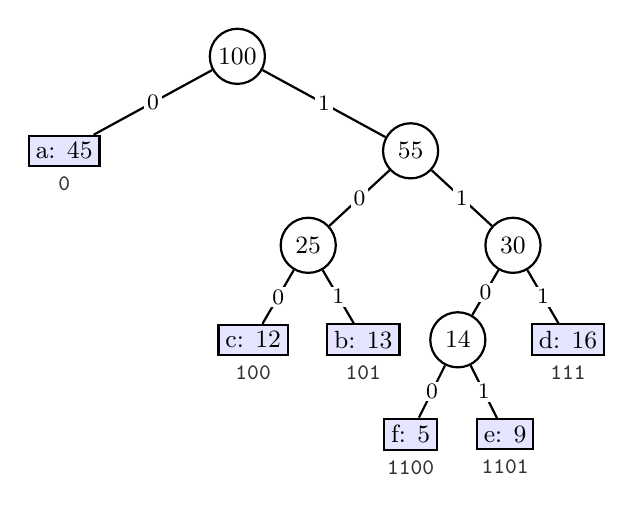
\begin{tikzpicture}[
  level distance=12mm,
  level 1/.style={sibling distance=44mm},
  level 2/.style={sibling distance=26mm},
  level 3/.style={sibling distance=14mm},
  level 4/.style={sibling distance=12mm},
  every node/.style={font=\small},
  inner/.style={circle, draw, thick, minimum size=7mm, inner sep=0pt},
  leaf/.style={draw, thick, fill=blue!10, inner sep=2.5pt},
  code/.style={label={[font=\footnotesize\ttfamily, gray!40!black]below:#1}},
  edge from parent/.style={draw, thick},
  bit/.style={font=\footnotesize, midway, fill=white, inner sep=1pt},
]
  % Merges: 5 + 9 = 14, 12 + 13 = 25, 14 + 16 = 30, 25 + 30 = 55, 45 + 55 = 100
  \node[inner] {100}
    child { node[leaf, code=0] {a: 45} edge from parent node[bit] {0} }
    child { node[inner] {55}
      child { node[inner] {25}
        child { node[leaf, code=100] {c: 12} edge from parent node[bit] {0} }
        child { node[leaf, code=101] {b: 13} edge from parent node[bit] {1} }
        edge from parent node[bit] {0} }
      child { node[inner] {30}
        child { node[inner] {14}
          child { node[leaf, code=1100] {f: 5} edge from parent node[bit] {0} }
          child { node[leaf, code=1101] {e: 9} edge from parent node[bit] {1} }
          edge from parent node[bit] {0} }
        child { node[leaf, code=111] {d: 16} edge from parent node[bit] {1} }
        edge from parent node[bit] {1} }
      edge from parent node[bit] {1} };
\end{tikzpicture}
